\documentclass[DM,lsstdoc,toc]{lsstdoc}
\usepackage{graphicx}
\usepackage{url}
\usepackage{latexsym}
\usepackage{color}
% black, blue, brown, cyan, darkgray, gray, green, lightgray, lime, magenta, blue, orange, pink, purple, red, teal, violet, white, yellow.
\usepackage{enumitem}

\title[LSST Special Programs]{Data Management \\ and LSST Special Programs}

\author{M.~L.~Graham, M.~Juri\'{c}, K.-T.~Lim, and E.~Bellm}

\setDocRef{DMTN-065}
\date{\today}
\setDocUpstreamLocation{\url{https://github.com/lsst-dm/dmtn-065}}

\setDocAbstract{This document provides an in-depth description of the role of the LSST Project in preparing software and providing computational resources to process the data from Special Programs (deep drilling fields and/or mini-surveys). The plans and description in this document flow down from the requirements in \citeds{LSE-61} regarding processing for Special Programs. The main target audience is the LSST Data Management (DM) team, but members of the community who are preparing white papers on science-driven observing strategies may also find this document useful. The potential diversity of data from Special Programs is summarized, including boundaries imposed by technical limitations of the LSST hardware. The capability of the planned Data Management system to processes this diversity of Special Programs data is the main focus of this document. Case studies are provided as examples of how the LSST software and/or user-generated pipelines may be combined to process the data from Special Programs.}

\setDocChangeRecord{%
\addtohist{1}{2017-11-14}{Status: internal working document.}{Melissa Graham}
\addtohist{1}{2018-06-17}{Updated to finalize and issue.}{Melissa Graham}
%\addtohist{2}{yyyy-mm-dd}{Future changes}{Future person}
}

\begin{document}

\maketitle

% CITATION EXAMPLES
% \verb|\citellp|: \citellp{LPM-17, LSE-30} \\
% \verb|\citell|: (SRD; \citell{LPM-17,LSE-29}) \\
% \verb|\citep[][]|: \citep[e.g.,][are interesting]{LPM-17,LSE-29} \\
% \verb|\cite|: \cite{LPM-17,LSE-29}



% % % % % % % % % % % % % % % % % % % % % % % % % % % % % % % % % % % %
\section{Introduction} \label{sec:intro}

The main LSST science goals will be met by the Wide-Fast-Deep (WFD) Main Survey, but this is expected to be accomplished with $85$--$90$\% of the observing time available over the $10$ year survey. The remaining $10$--$15$\% of the time will be spent on Special Programs: alternative survey areas and/or observing strategies driven by a specific science goal. A call for white papers that provide scientific motivation and observing strategies for the WFD survey and Special Programs, \citeds{Document-28382}, released in June 2018, has a deadline of November 30 2018. It is conceivable that Special Programs might obtain imaging data that are significantly different from the WFD main survey, and/or requires special processing in order to achieve the program's science goals. This document provides an in-depth description of the role of the LSST Project in preparing to process the data from Special Programs (expanding on the general description in Section 6 of \citeds{LSE-163}). The main target audience is the LSST Data Management (DM) team, but members of the science community who are preparing white paper proposals may also find this document useful.

{\bf Special Programs Terminology -- } The WFD main survey will survey the sky with a series of {\bf visits}, and each field will be visited $>800$ times over $10$ years. A {\bf standard visit} is composed of $2\times15$ second exposures (commonly referred to as ``snaps") and an {\bf alternative standard visit} is composed of a single $30$ second exposure. A {\bf non-standard visit} is any other exposure time(s) or number of snaps. Special Programs are typically divided into two types: {\bf Deep Drilling}, a single pointing for which many exposures are obtained in a relatively short amount of time (e.g., $>2\times$ as many visits in six months as the WFD will obtain in 10 years); and {\bf Mini-Surveys}, which refer to either new sky areas observed with a WFD-like survey, or sky areas within the WFD but observed with a specialized strategy. 

{\bf The LSST Project's Role in Processing Special Programs Data -- } The formal requirements regarding LSST's role in processing Special Programs data are in \citeds{LSE-61}, and the following statements have been derived from those requirements. The LSST Project will not take formal responsibility for specialized data reduction algorithms needed to process data, including images taken in non-standard modes. The term "specialized algorithms" refers to software that is not already within scope of the LSST Data Management (DM) science pipelines, and may include, for example: difference imaging for short exposures in which the PSF is not well-formed, shift-and-stack for faint moving objects, or any software with computational needs that significantly surpass the processing budget per image (compared to the processing of a WFD image). The Project will incorporate Special Programs data into the Prompt and/or Data Release processing pipelines and data products of the WFD Main Survey, such as {\tt Alerts}, {\tt CoAdds}, or {\tt Source} and {\tt Object} catalogs (with appropriate flags; LSST data products are described in \citeds{LSE-163}), whenever this (1) can be accomplished with existing software, and (2) is scientifically beneficial to that data product. The Project will also reconfigure its pipelines to generate separate imaging and catalog data products for Special Programs, whenever this can be accomplished with existing software. Finally, the Project will enable user-generated processing via the Science Platform (\citeds{LSE-319}), which will provide software tools and computational resources for (re)processing LSST data.

{\bf Document Overview -- } The purpose of this document is to assess the potential diversity of imaging data that might be obtained by Special Programs (Section \ref{sec:data}), and to explore and clarify whether -- and to what extent -- DM's planned pipelines and user services will be able to handle this diversity of data (Section \ref{sec:dmplans}). As described in the call for white papers on cadence optimization (\citeds{Document-28382}), Special Programs that may require specialized or computationally-intense algorithms to meet their science goals are required to describe how these processing needs will be met. Sections \ref{sec:data} and \ref{sec:dmplans} have been designed to help white paper authors figure out whether their proposed Science Program(s) require processing that would be considered out of DM's scope, and in Section \ref{sec:SPCS} we have provided a series of science-driven case studies as examples. 

% In Appendix \ref{sec:docrev}, we endeavor to ensure that the DM's plans for Special Programs processing are appropriately expressed in all of the major Project documents and that the computational system and human work-hours needed to accomplish Special Programs processing have been accurately evaluated. This content will only be of interest to the DM team.



% % % % % % % % % % % % % % % % % % % % % % % % % % % % % % % % % % % %
% % % % % % % % % % % % % % % % % % % % % % % % % % % % % % % % % % % %
% % % % % % % % % % % % % % % % % % % % % % % % % % % % % % % % % % % %
\clearpage
\section{The Potential Diversity of Special Programs Data} \label{sec:data}

To define the extent to which Data Management will be able to process data from Special Programs, a comprehensive understanding of the potential diversity of data from Special Programs -- compared to the WFD's sky survey of standard visits -- is needed. 

To build up this comprehensive understanding, in Section \ref{ssec:data_bounds} we considered any technical limitations that the facility and instrumentation will or might place on the data. We find that the hardware imposes few boundaries on how data can be obtained, but that a high number of filter changes and/or long slews are inefficient due to their large overheads. The minimum exposure time is $1$ second (stretch goal: $0.1$ seconds), but there is currently a technical boundary that limits the readout rate to $1$ every $15$ seconds.

Next, we considered the Special Programs that have been openly discussed so far in the Science Community (Appendix \ref{sec:data_prev}). Based on this consideration, most of the proposed Special Programs are likely to use visits that are similar to the WFD Main Survey, but some will require exposures that are significantly shorter, or that are obtained with a bright sky background during twilight. The cadence and patterns may also differ from the WFD main survey, such as long series of exposures obtained of the same field (i.e., deep drilling), or a strategy optimized to find very fast-moving objects. In addition, images of very crowded fields in the Galactic Plane may be included (at all or more often than the WFD Main Survey). It does not appear that any of the previously proposed Special Programs violate the hardware-imposed boundaries discussed in Section \ref{ssec:data_bounds}.

% % % % % % % % % % % % % % % % % % % % % % % % % % % % % % % % % % % %
\subsection{Hardware Boundaries}\label{ssec:data_bounds}

Here we consider the technical boundaries on the diversity of data products that are expected to (or may) be imposed by limitations from the camera, telescope, and/or site (boundaries imposed by DM processing capabilities are considered in Section \ref{sec:dmplans}). 

{\bf Filter Changes -- } The maximum time for filter change is $120$ seconds: $30$ seconds for the telescope to reorient the camera to its nominal zero angle position on the rotator, and $90$ seconds to the camera subsystem for executing the change (OSS-REQ-0293; \citeds{LSE-30}). Assuming that most Special Programs would be designed to keep overheads $<100\%$ and would be using standard $30$ second visits, the filter change time indicates that it is likely that at least $4$ exposures in a given filter would be obtained between filter changes -- but this is not actually a technical boundary. 

{\bf Filter Carousel Loads -- } As described in \citeds{Document-28382}, the filter carousel can hold five of the six LSST filters at a time, and filter loads are done in the day. The system is designed to support $3000$ loads and $100000$ filter changes in $15$ years, which is an average of $17$ changes per night (after accounting for filter changes during calibrations). Individual filters will support $30000$ changes in $15$ years. Based on these technical boundaries, we know that there will never be data in more than five filters in a given night.

{\bf Exposure Times -- } The minimum exposure time is $1$ second, with a stretch goal of $0.1$ seconds (OSS-REQ-0291; \citeds{LSE-30}). The maximum exposure time is not restricted. The readout time is $2$ seconds, and would be significant overhead on short exposures. Images with exposure times $<15$ seconds may still have to be separated by $15$ seconds for thermal tolerance; i.e., that the minimum readout rate is one image every $15$ seconds, regardless of exposure time (OSS-REQ-0291; \citeds{LSE-30}). We therefore consider the $15$ interval between images a technical boundary on the potential diversity of data products.
% $\bullet$ However, for exposure times there are other considerations. The minimum exposure time needed to create an image with a PSF that is well-formed enough for difference imaging is a separate question. Changing the exposure time also affects the photometric and astrometric calibrations. Assuming a 1 second exposure can be reduced and calibrated, its detected point sources will span $13 < r < 21$ magnitudes, whereas a 15 second exposure saturates at $r\sim15.8$ mag. A 150 second image would saturate at $r\sim18.3$, perhaps leaving too few stars overlapping with e.g., templates or WFD images, for astrometric and photometric calibrations. Additionally, the impact on CR rejection routines is untested for long exposures.

{\bf Telescope Slew -- } As described in \citeds{Document-28382}, large slews would have considerable overheads, but there are no technical boundaries on the size of a single slew or the accrued slew distance.

{\bf Camera Rotation -- } There requirements on the rotator's capabilities do not set any limits on the per-night or total lifetime rotation (OSS-REQ-0301, -0300; \citeds{LSE-30}) which might put boundaries on the distance between successive visits or the ability to jump between two widely separated fields. JIRA ticket DM-12573 is currently open and asking for clarification from the camera team on this. Until then, we assume there are no technical boundaries imposed by camera rotation constraints on the potential diversity of data products. 


% % % % % % % % % % % % % % % % % % % % % % % % % % % % % % % % % % % %
% % % % % % % % % % % % % % % % % % % % % % % % % % % % % % % % % % % %
% % % % % % % % % % % % % % % % % % % % % % % % % % % % % % % % % % % %
\clearpage
\section{Processing Special Programs Data with LSST DM Pipelines} \label{sec:dmplans}

In this section we go into greater detail regarding the Projects' role in processing data from Special Programs, as introduced in Section \ref{sec:intro}. We discuss the ability of the planned DM pipelines to: process diverse imaging data that are unlike the WFD's standard visits in Section \ref{ssec:dmplans_NSV}; incorporate Special Programs data into the Prompt and Data Release pipelines and data products for the WFD main survey in Section \ref{ssec:dmplans_WFD}; reconfigure the pipelines and generate unique sets of data products for each Special Program in Section \ref{ssec:dmplans_reconfig}; and enable user-generated pipelines and data products in Section \ref{ssec:dmplans_user}.

% % % % % % % % % % % % % % % % % %
\subsection{Processing Diverse Imaging Data Unlike the WFD Main Survey}\label{ssec:dmplans_NSV}

As described in Section \ref{sec:data}, Special Programs will be able -- and likely -- to request observing modes with shorter (or longer) exposure times, long sequences of visits to the same field, and/or imaging of very crowded fields. We review the capability of DM's planned pipelines to process such each of these kinds of diverse data, keeping in mind that the processing boundaries might ultimately be defined not by what is technically possible, but by the resulting image quality parameters such as the number of stars with sufficient flux for photometric calibration or the source area density (crowding). Furthermore, that these boundaries imposed by the data quality might not be constrained until the final performance of DM's algorithms, as described in the Data Management Applications Design (\citeds{LDM-151}) document, is fully characterized.

\subsubsection{Exposure Times}

Images which deviate significantly from the $15$ second duration for the WFD main survey may encounter issues in the instrument signature removal routine, in the correction for differential chromatic refraction, in the difference imaging analysis pipeline, and/or in the photometric and astrometric calibrations due to a differently sampled set of standard stars per CCD. We discuss shorter and longer exposure in turn.

\textbf{Shorter Exposures.} The camera constraint on the minimum supported exposure time is currently 1 second (stretch goal 0.1 seconds). The minimum exposure time for an image to be successfully reduced with Instrument Signature Removal (ISR) is under consideration (see JIRA ticket DM-12574). Assuming that 1 second exposure can be reduced and calibrated, its detected point sources will span a dynamic range of $r \approx 12.9$ -- $21.0$ magnitudes. A template image built on $15$ second exposures will saturate at $r \approx 15.8$, but this still leaves stars between $15.8$--$21.0$ magnitudes to be used in the PSF-matching (and all other filters have a similarly large overlap). However, in order for an image to be successfully PSF-matched to the template, the PSF must be well formed (no speckle pattern), and have a spatial variance that the pipeline is capable of modeling (be smoothly varying on some minimal scale). As a simple demonstration, Figure \ref{fig:expt} shows that perhaps exposure times shorter than $2$ seconds do not have a well-formed PSF (using the centroid of a 2D Gaussian fit as a proxy for "well-formed"). The minimum exposure time for an image to be successfully processed by the Difference Imaging Analysis (DIA) pipeline is currently under consideration (see JIRA ticket DM-12574).

\begin{figure}
\begin{center}
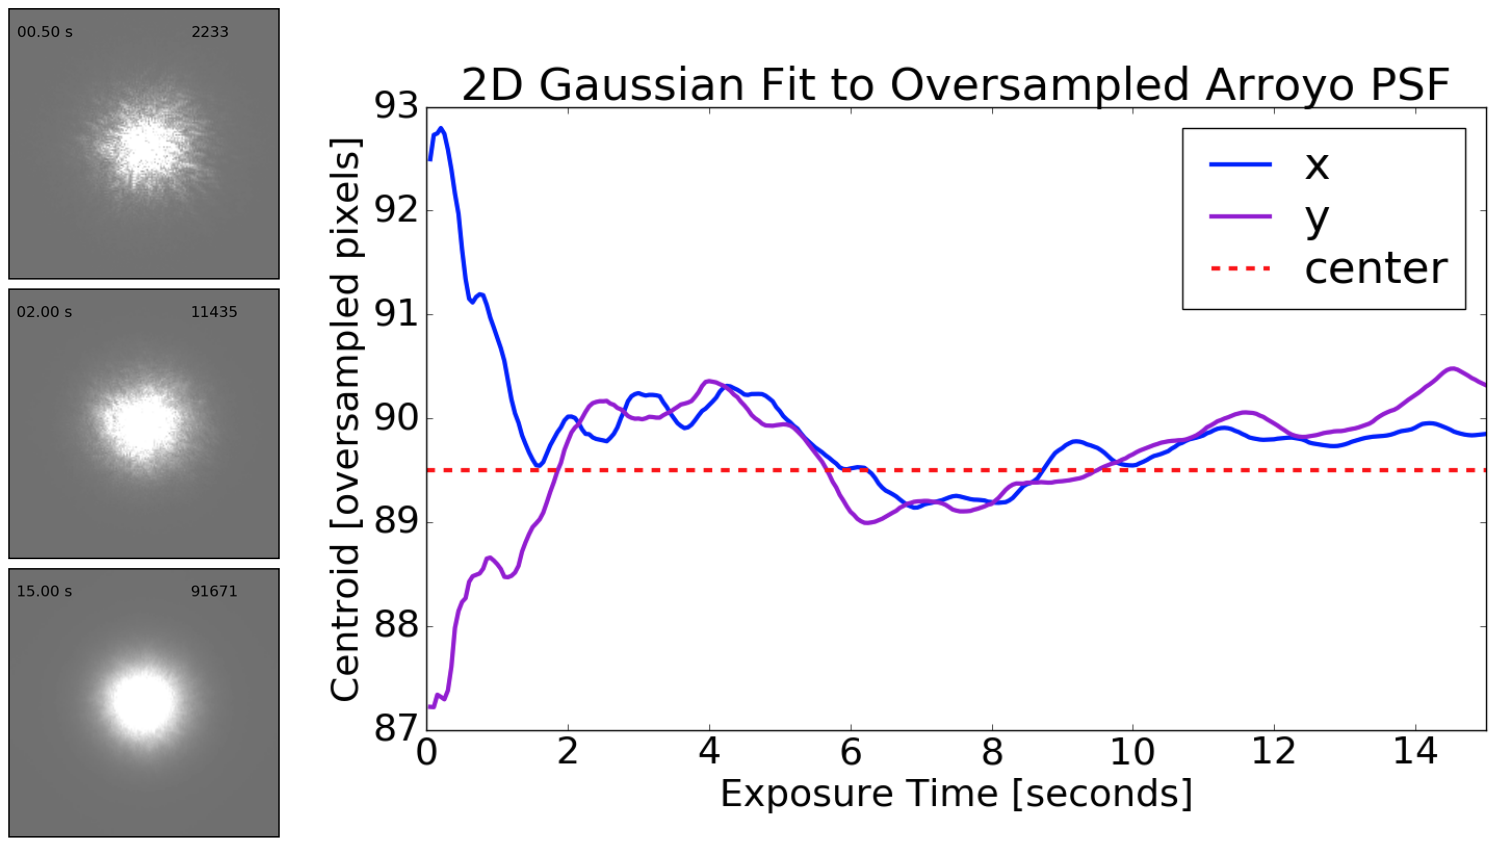
\includegraphics[width=14cm,trim={0cm 0cm 0cm 0cm}, clip]{figures/exptime.png}
\caption{At left, Arroyo atmosphere-only simulated PSF for LSST (with oversampled pixels) with exposure times of 0.5, 2, and 15 seconds (top to bottom), courtesy of Bo Xin. At right, blue and purple lines show the location of the centroid derived from a 2D Gaussian fit to the PSF as a function of exposure time, with the red dashed line showing the true center. We can see that for exposure times greater than 2 seconds, the centroid converges near its true value. \label{fig:expt}}
\end{center}
\end{figure}

\textbf{Longer Exposures.} There is no maximum exposure time specified for an LSST image. Given that the template image will be a stack of at least a year or two of data, processing a $5$--$10$ times deeper single image through the difference imaging pipeline should be fine. However, a $2\times150$ second exposure would saturate at $r \approx 18.3$, and cosmic-ray rejection completeness might suffer (unknown), which could impact the quality of a difference image and the detected sources. Additionally, any system qualities that vary on short (but $>30$ second) timescales could inhibit photometric calibration (e.g., tracking). A potential maximum exposure time from a processing perspective is currently under consideration (see JIRA ticket DM-12574).

% In conversation with DM-AP team members (Reiss, Findeisen, Connolly, Bo) there has not yet been a study of the safe range of exposure times that will be allowed to contribute to the Level 1 and Alert Stream. One possibly useful study is Chang et al. (2012), "Atmospheric point spread function interpolation for weak lensing in short exposure imaging data". They show that a 15 second exposure contains PSF variability on short spatial scales across a 1 square degree image which, for extragalactic fields with few stars (i.e., but good for weak lensing), is hard to characterize. They present a new software package to do mitigate the effects. Alternatively, we may need to use software packages \texttt{PhoSim} (Peterson et al. 2015; \citep{2015ApJS..218...14P}) or \texttt{ARROYO} \citep{2004SPIE.5497..290B} to at least simply characterize the PSF stability as a function of exposure time.
% In conversation with K.-T., exposure times of 10 to 120 seconds will not be a problem for the processing pipeline to accommodate, but the ingest rate of images and the number of exposure per visit are the aspects that could cause issues (discussed below).
% Is it conceivable that the LSST would spend time on a Special Program that will acquire short exposures if DM's algorithms cannot be shown to adequately reduce and calibrate them? This is probably best left ot a policy issue (beyond the scope of this document).

\subsubsection{Number of Exposures per Visit (Long Sequences of a Single Field)}

There is no processing constraint on the number of consecutive exposures that could be obtained of a single field. From a DM perspective, it would be best if these exposures were packaged into visits of no more than 2 exposures per visit, to minimize the need to reconfigure of the pipelines, and because the camera only ``clears" between visits. 

% K.-T. Lim has pointed out that an odd number of exposures is a non-standard visit; two snaps is hardwired into the code. This is baked-in to a configuration so that the pipeline can have a definition of what kind of timing delay constitutes ``late".  Moving away from 2 exposures per visit requires a configuration change to the pipelines, which incurs an overhead (up to 1 minute) -- in fact, K.-T. things that between $10$ and $120$ seconds exposure times can easily be handled by the pipeline (i.e., can be run through ISR using scaled calibration frames), so long as they come in pairs. The real problem is knowing how long the processing should take, and not killing a process that is taking longer because there were 4 snaps in the visit instead of 2. To accommodate non-standard visits requires that the scheduler pass on the information of the number of snaps in the visit (\ref{DMSR-1}). Then the processing pipeline will know to, e.g., not attempt to difference the two snaps in the case were there is an odd number of snaps in a visit. \textit{MLG -- I've heard rumors of a CR regarding alternate standard visits of $1\times30$ seconds, but do not know the status or implications of this.}

% K.-T. has also pointed out that currently, a deep drilling field would be interpreted as a single visit of 50 exposures by the scheduler. One implication of this is that since the camera only ``clears" prior to a new visit, it would not do this for the entire 50-exposure sequence. The processing pipeline would need to know how to divide this sequence up into visits. As there is no current requirement for DM to receive the information that the scheduler is about to do a 50 exposure visit, we need \ref{DMSR-1} to add the proposal ID and the number of exposures per visit to the meta data, and then it should be OK for DM to parse this visit information in the reduction pipeline.

\subsubsection{Images in Very Crowded Fields}

The LSST pipelines' performance in crowded fields is documented in \citeds{DMTN-077}, which finds that, e.g., in Galactic Plane regions with a source density of $500000$ sources per square degree, the completeness drops to 50\% at $20.2$ magnitudes. The slide deck at \citeds{Document-27962} also describes DM's plans for processing crowded fields. These may or may not be appropriate for Special Programs data, depending on the science goals.


% % % % % % % % % % % % % % % % % %
\subsection{Including Special Programs Data in the WFD Main Survey's Data Products}\label{ssec:dmplans_WFD}

As described in Section \ref{sec:intro}, the Project may incorporate Special Programs data into the WFD main survey's pipelines and data products whenever this is (1) possible and (2) scientifically beneficial. This will likely be at the discretion of the data quality assessment team during Operations. In the following three sections we project when and how Special Programs data might be incorporated into the pipelines and data products of the Prompt pipeline and the Alert stream (Section \ref{ssec:dmplans_prompt}) and the annual Data Release pipeline (Section \ref{ssec:dmplans_drp}).

\subsubsection{The Prompt Pipeline and Alert Generation}\label{ssec:dmplans_prompt}

It would be beneficial to transient science to include as many LSST images into the Difference Imaging Analysis (DIA) pipeline and the Alert Stream as possible. Only images that can be processed with the Prompt DIA pipeline with the $60$-second timeline can contribute to the Alert Stream. As discussed in Section \ref{sec:data}, this might prohibit exposures shorter than $<15$ seconds and/or visit cadences shorter than $1$ per $\sim30$ seconds. This might also prohibit the inclusion of very crowded fields that require more computational resources. A field must have an LSST template image to be processed by the DIA pipeline, which would prohibit immediate Alerts from new survey fields. It should be possible to load and use an alternative template image (than what would be used for that field if and when it is covered by the WFD main survey) in the Prompt pipeline for fields from a Special Program. 

There may be a couple of issues encountered with Alerts from many consecutive visits of Deep Drilling fields. One is that, since the Alert contains the full record of all associated {\tt DIASources} from the past 12 months (\citeds{LSE-163}), for a Deep Drilling Field with significantly more visits over the year, the size of the Alert might become prohibitively large (TBD). Another is that the self-consistency of the \texttt{DIAObjects} catalog may suffer during consecutive visits of a single field. For example, the processing for image $2$ of a sequence would begin when the processing for image $1$ is only halfway complete. Any new {\tt DIASource} in image $1$ that cannot be associated (by coordinate) with an existing {\tt DIAObject} becomes a new {\tt DIAObject}. When this source is again detected in image $2$, another new {\tt DIAObject} would be created if the catalog has not yet been updated. The best solution might be to flag {\tt Alerts} which may suffer from incomplete {\tt DIASource}--{\tt DIAObject} associations (see JIRA ticket DM-12574). 

% \textbf{Templates:} The template images that are used in the Level 1 difference imaging pipeline will be built from the Level 2 DRP, and so the first factor affecting a Special Programs image's suitability for Level 1 is to be in a region of sky with an existing template. So long as there is a template, when the exposure time is equivalent to a WFD visit image, $\sim 30$ seconds, treating the image as Level 1 is going to be fine. When processing Special Programs data with the Level 1 pipeline, certain science cases might call for the capability to load and use a certain template that is different from the WFD template (i.e., built over a different timescale). K.-T. confirms that there is not enough memory allotted to store more than one template over the whole sky, but for sub-regions, storing and using an alternative template should be possible. This is not an issue limited to Special Programs, since during commissioning it is conceivable that multiple template versions. K.-T. also confirms that the capability for the processing pipeline to choose a given template based on the programID in the raw image metadata will exist.

% \textbf{Processing backup:} Are there options for short-term increases in parallel processing power at NCSA? (Such options might be needed anyway to process crowded fields with $>$10k \texttt{DIASources}.) The bandwidth needed to load templates at a faster rate is also a concern, since templates have twice as many pixels, if the data acquistion rate is surveying at twice the WFD main survey rate, that's a $4\times$ additional bandwidth load. However, at NCSA there should be ways to elastically change the amount of processing power available. This is also an issue for crowded fields (below).

% Special Programs are more likely to include crowded fields than the WFD main survey area. Due to the increased number of sources, the number of \texttt{DIASources} -- and therefore the number of Alerts -- increases as well. In turn, this increases the processing time and in some cases, may exceed the 60 second limit for Alert Production. A policy is needed on whether Alerts from crowded fields should be allowed a delay, or allowed to be incomplete. K.-T. reports that the control system can easily kill processes that are running over time and move forward with existing outputs -- but that perhaps it will be just as easy to let it keep running and elastically grab additional NCSA resources as needed. This appears possible because the batch system is larger than the Level 1 allocation, although we might not know that this is possible until Level 1 integration happens at NCSA (see Document LDM-230, the operations concepts).

{\bf The Moving Object Processing System (MOPS) -- } Since MOPS takes \texttt{DIASources} as input, any Special Programs images that can be run through the Alert Pipeline can be ingested by MOPS. As discussed under "Solar System Objects (SSO)" in Appendix \ref{sec:data_prev}, most of the Special Programs data associated with SSO science will obtain standard visit images anyway. %There was some concern that a large number of small-separation sources might overwhelm the processing system (i.e., from a deep drilling field with many exposures in a sequence), but upon further consideration this worry was rejected.

\subsubsection{The Data Release Pipeline (DRP)}\label{ssec:dmplans_drp}

This document is not the place for a full consideration of whether or not it would be ``scientifically beneficial" to include any Special Programs data in the DRP data products -- namely, the deep image CoAdds and their corresponding {\tt Source} and {\tt Object} catalogs (\citeds{LSE-163}) -- and we leave that decision for the data quality assessment team in LSST Operations. One example might be when Special Programs data brings additional area up to the same level of depth and cadence as the rest of the WFD main survey. Another may be if including some or all of the shallower Galactic Plane coverage suppresses edge effects or low-order modes in the all-sky photometric solutions.

% % % % % % % % % % % % % % % % % %
\subsection{Reconfiguring DM Pipeline Components for Special Programs}\label{ssec:dmplans_reconfig}

Whether or not Special Programs images are incorporated into the WFD main survey's data products, it is anticipated that most of the Special Program's science goals will require (or benefit from) separate data products (i.e., CoAdds and/or catalogs). For this reason, LSST intends to reconfigure the DM's pipelines in order to generate unique and separate -- but joinable -- imaging and catalog products for Special Programs data, whenever possible. In this context, ``possible" means that no new algorithms need to be written and that an intensive amount of additional computational resources is not required for the processing.

In a ``possible" scenario, DM would assemble a pipeline from existing DM codes in order to process data associated with a given Special Program and build image and catalog products that meet the science needs of that particular program. For example, for a DDF SN survey (see Section \ref{ssec:SPCS_SNDDF}), existing DM codes would be used to: (1) make a deep template image from a certain time window, (2) process standard single visit images, (3) create a nightly CoAdd, (4) run difference imaging analysis, (5) run source detection on the difference images, and (6) create \texttt{DIASource} and \texttt{DIAObject} catalog equivalents (this example is also given in Section 6 of the \DPDD, \citedsp{LSE-163}). This type of reconfiguration would also be possible to create as a user-generated pipeline (Section \ref{ssec:dmplans_user}), but having these products provided by the Project ensures a consistent and verified level of quality. %, as well as access for all users to the processed Special Programs data products, which would only increase the scientific value of Special Programs data. --> MLG: data rights doc will probably state that the products for SP data that is only processed by user-generated pipelines will have to be served to all users

The above statements of intent are derived from the Data Management Subsystem Requirements document, \citeds{LSE-61}, which contains several requirements related to the processing of data from Special Programs (DMS-REQ-0069, 0320, 0321, 0322, and 0344). To ensure that the work-hours needed to reconfigure and test the pipelines, and run them and verify the data products for public release (which may potentially be needed on intermediate timescales that do not coincide with the Prompt/Yearly timescales, e.g., monthly stacks of deep drilling fields), have been included in the personnel budget, JIRA ticket DM-12575 is currently under consideration. 

DMS-REQ-0320 states that "it shall be possible for special programs to trigger their own data processing recipes". A header keyword identifying an image as related to a Special Program would be sufficient to send it to a dedicated processing pipeline, and would satisfy this requirement. JIRA ticket DM-12576 is currently open to make sure that this happens. 


% % % % % % % % % % % % % % % % % %
\subsection{Support for User-Driven Processing of Special Programs Data}\label{ssec:dmplans_user}

In cases where the science goals of a Special Program require specialized algorithms and cannot be achieved by reconfiguring DM's software, then user-generated pipelines will be needed. Towards this end, LSST DM is making all of its software open-source, and preparing the Science Platform (\citeds{LSE-319}), through which users can access the tools and computational resources to assemble data processing pipelines to achieve their science goals (whether related to Special Programs data or not). During Operations, there will be a method for the system to allocation processing resources in the case of over-subscription. JIRA ticket DM-12577 is currently open to inspire an investigation of whether additional Science Platform capabilities are needed to enable user-driven processing of Special Programs data.

If the user-generated processing pipeline for Special Programs data requires requires significantly more computational resources than have been allocated -- where that allocation has been sized approximately, based on image processing for WFD main survey data (i.e., difference imaging, source detection, and/or stacking) -- then external computational resources may be necessary. To support such external processing DM intends to make the data and its code base accessible to and exportable by users in the science community.

No user-generated pipeline may contribute Alerts to the Alert Stream, although a separate stream should be possible if the packet and transport formats are adopted (see also Section \ref{ssec:dmplans_user}).

It is furthermore expected that, over time, some user-designed pipelines might become ``adopted", installed and operated (and change controlled) by the LSST Operations team. For both adopted and user-run code, whether they are for Special Programs or WFD survey data, the LSST DM team will encourage and facilitate data product databases that are built with the same schema as -- and can easily be joined with -- the tables of the Prompt and DRP data products. An alternative option to ``adopted" code is ``adopted" data products: situations in which user-generated code is run externally, a data catalog is returned to LSST to be ingested, verified, and made public. JIRA ticket DM-12578 is currently open to consider the staffing needs and process for adopting user-generated code or products; this issue is not necessarily limited to Special Programs. 


% % % % % % % % % % % % % % % % % % % % % % % % % % % % % % % % % % % %
\clearpage
\section{Special Programs Processing Case Studies}\label{sec:SPCS}

For further insight to the DM-related needs of potential Special Programs, we can write out all of the data acquisition and processing steps, in order, that some of the proposed Special Programs might use. This kind of thought experiment of describing the reductions and processing could also be a required section of all future white paper proposals. Note that we are not including any analysis in these descriptions, only processing and products. These are not necessarily complete and may even be incorrect in some places, as we are not experts in the science needs of these potential Special Programs; they could use some more thought and input.

Basic steps that we use to describe a processing case study: \\
Step 1. Data Acquisition. \\
Step 2. Inclusion in the Prompt Pipeline and Alert Generation. \\
Step 3. Delivery of LSST Processed Images. \\
Step 4. Reconfigured Processing Pipelines and Separate Data Products. \\
Step 5. Inclusion in the DRP Data Products for the WFD Main Survey. \\
Step 6. User-Generated Pipelines and Products. \\


% % % % % % %
\subsection{Searching for TNOs with Shift-and-Stack}\label{ssec:SPCS_TNO}

This Special Programs processing summary is based on Becker et al. (2011) white paper to find TNOs with shift-and stack (SAS) \citedsp{Document-11013}.

Step 1. Data Acquisition. \\
The observational sequence is triggered. In a single night, the 9 adjacent fields in a 3x3 grid are observed with $336$ $\times$ $15$ second $r$-band exposures. This sequence is always repeated 2-3 nights later. This re-visit sequence is repeated 3 more times: 1.5 months, 3 months, and 13.5 months later. Data obtained in the $g$-band filter is also acceptable. \citedsp{Document-11013}

Step 2. Inclusion in the Prompt Pipeline and Alert Generation. \\
Each $2\times15$ second visit is processed in the Prompt pipeline and Alerts are released within 60 seconds.

Step 3. Delivery of LSST Processed Images. \\
The raw, reduced, and calibrated exposures and difference images from the Prompt pipeline are made available within \texttt{L1PublicT} (currently 24 hours; LSR-REQ-0104), but this is not very relevant for this program, which requires a year of dispersed observations before the processing pipelines for SAS can be run.

Step 4. Reconfigured Processing Pipelines and Separate Data Products. \\
Shift-and-stack processing is beyond the scope of DM's algorithms.

Step 5. Inclusion in the DRP Data Products for the WFD Main Survey. \\
As with all Special Programs data, they might be included in the products of the WFD main survey if DM decides it is beneficial. However, since these images are much deeper than stacks made from the WFD survey, and the strict timing of the observations might lead to their acquisition in sub-optimal conditions, it is unlikely that they would \textit{all} be incorporated.

Step 6. User-Generated Pipelines and Products. \\
The user-generated pipeline running the shift-and-stack processing will be set up and submitted for batch processing by the user through the Science Platform or on an external processor. Pipeline inputs will be the 336 processed exposures per field per re-visit sequence. The DRP difference imaging routine will be used with the same template tract/patch for all. Custom, user-generated algorithms will shift the exposures and create difference images, then DRP routines can stack and do source detection and characterization and generate an object database. Custom code will derive orbital parameters for the detections and add them to a {\tt SSObjects}-like database.


% % % % % % %
\subsection{Searching for Supernovae in Deep Drilling Fields}\label{ssec:SPCS_SNDDF}

Step 1. Data Acquisition. \\
On a single deep drilling field, the scheduler obtains e.g., 5, 10, 10, 9, and 10 visits with $2\times15$ second exposures in $grizy$ (or similar for the night's filter set) and a small dither pattern between visits.

Step 2. Inclusion in the Prompt Pipeline and Alert Generation. \\
Each $2\times15$ second visit is processed by the Prompt pipeline's DIA, and Alerts are released within 60 seconds. They are flagged to denote the image source is a DDF and that source association might be compromised.

Step 3. Delivery of LSST Processed Images. \\
The raw, reduced, and calibrated exposures and difference images from the Prompt pipeline are made available within \texttt{L1PublicT} (currently 24 hours; LSR-REQ-0104).

Step 4. Reconfigured Processing Pipelines and Separate Data Products. \\
The required data products for this science goal can be met by reconfiguring the DM pipelines. First, a template image for the field will be made using DM stacking algorithms. On nights when this DDF is observed, at the end of the sequence of observations, DM algorithms are used to create a nightly deep stack, PSF-match it with the template, create a deep difference image, run source detection on the differences, and create separate databases of \texttt{DIAObject}, \texttt{DIASource}, and \texttt{Object} that are unique to this DDF. The LSST codes for alert packet and transport could be used to distribute the detected objects e.g., to the same brokers that receive the Alert Stream, or alternative destinations. However, these packets would not be distributed via the LSST {\tt Alert Stream}, and would need to be identified as, e.g., DDF Alerts. Note that JIRA ticket DM-12585 is currently open to investigate whether or not the internal real/bogus routine be able to run on a nightly CoAdd of deep drilling difference images.

Step 5. Inclusion in the DRP Data Products for the WFD Main Survey. \\
As with all Special Programs data, they might be included in the products of the WFD main survey if DM decides it is beneficial.

Step 6. User-Generated Pipelines and Products. \\
For the science goal of searching for supernovae in nightly stacked DDF images, no separate user-generated software appears necessary.


% % % % % % %
\subsection{A Twilight Survey with Short Exposures}\label{ssec:SPCS_Twilight}

Several kinds of twilight surveys with short exposures have been or might be proposed: to put brighter stars (or transients such as supernovae) that saturate in a $15$ second image onto the LSST photometric system and/or to observe the Sweetspot, 60 degrees from the sun, for near-Earth objects. The processing case study for these is currently limited by unknowns about the first step: the reduction of processed single visit images.

Step 1. Data Acquisition. \\
At a specified time (or e.g., 6 degree twilight), the scheduler begins dither pattern of short exposures. Location and exposure times are set by the sky brightness and desired saturation limits.

Step 2. Inclusion in the Prompt Pipeline and Alert Generation. \\
Pending studies of short-exposure suitability for DIA (see Section \ref{ssec:dmplans_NSV}) and scalable processing capabilities to incorporate a faster image-input rate than $1$ every $30$ seconds, these data could {\it potentially} be incorporated and spawn Alerts.

Step 3. Delivery of LSST Processed Images. \\
Pending the issues mentioned above, the raw, reduced, and calibrated exposures and difference images from the Prompt pipeline are made available within  \texttt{L1PublicT} (currently 24 hours; LSR-REQ-0104).

Step 4. Reconfigured Processing Pipelines and Separate Data Products. \\
This is officially not determined, but so long as the short-exposure images can be processed and have enough stars for photometric and astrometric calibration, reconfigured DM pipelines will probably be sufficient for creating image and catalog products from this kind of data.

Step 5. Inclusion in the DRP Data Products for the WFD Main Survey. \\
These short-exposure, high sky background images would not contribute to the DRP data products created for the WFD survey.

Step 6. User-Generated Pipelines and Products. \\
If short-exposure images cannot be processed with the existing DM algorithms, a user-generated processing pipeline might be needed to reduce the raw data. 

Side note: A short-exposure survey of the bright stars of M67, described in Chapter 10.4 of the Observing Strategy White Paper \citep{2017arXiv170804058L}, suggests using the stretch goal of 0.1 second exposures or, if that is not possible, \textit{"custom pixel masks to accurately perform photometry on stars as much as 6 magnitudes brighter than the saturation level"}. This would be considered a user-generated algorithm.


% % % % % % %
\subsection{The Galactic Plane Survey for Variable Stars and/or Exoplanets}\label{ssec:SPCS_GPVSEx}

Step 1. Data Acquisition. \\
The schedule incorporates fields in the Galactic Plane, and executes $2\times15$ second visits in these fields (or shorter, for a shallower depth than the WFD main survey).

Step 2. Inclusion in the Prompt Pipeline and Alert Generation. \\
Each $2\times15$ second visit is processed in the Prompt pipeline and Alerts are released within 60 seconds. Extremely crowded fields might have to be skipped if they take longer to process and violate the $60$ second latency for Alerts. 

Step 3. Delivery of LSST Processed Images. \\
The raw, reduced, and calibrated exposures and difference images from the Prompt pipeline are made available within  \texttt{L1PublicT} (currently 24 hours; LSR-REQ-0104).

Step 4. Reconfigured Processing Pipelines and Separate Data Products. \\
The image and catalog products needed for science with the Galactic Plane are very similar to the products of the Prompt and DRP pipelines, so it seems that not much reconfiguration would be needed. The biggest difference might be the incorporation of a user-supplied deblender algorithm optimized for very crowded fields.

Step 5. Inclusion in the DRP Data Products for the WFD Main Survey. \\
It is quite likely that images from the Galactic Plane will be included into the products of the WFD main survey, as they could e.g., reduce edge effects and help with global photometric classification, but this will depend on deblender performance, and left to the discretion of DM. 

Step 6. User-Generated Pipelines and Products. \\
It seems likely that science users will want to deploy their alternative deblending algorithms on this data set and create their own catalogs.

%% % % % % % %
\subsection{A More General Level 3 Shift-and-Stack Case Study, by Mario}\label{ssec:SPCS_SAS}

A Level 3 processing case study for shift-and-stack on a large number images. By Mario.

\#1. The scheduler is configured to repeatedly (e.g., 10 times) observe a field during the same night with longer exposure than usual (e.g., 120 sec). [ and we should take the actual numbers from the TNO-DDF whitepaper; don't have the internet right now or I would].

\#2. The images are processed as regular "Level 1" products within 60 seconds, and transmitted as alerts, with results stored into the regular L1 database. This will happen automatically for all images (perhaps within some range of exposure times?).

\#3. The raw images (and all necessary calibrations), calexps, and standard L1 diffims are made available within 10 minutes to the batch system for processing with special programs-specific codes. This is the same batch system we make available to the users for running Level 3 codes [Q for us: is it? or is is the same one that's used to process calibrations? have these systems been sized?].

\#3 a). The code running the shift-and-stack processing will be externally developed and delivered, but will be installed and operated (and change controlled!) by the LSST Operations team. That is, we don't expect someone external to the ops team to babysit the code on a nightly basis. In fact, it's the opposite: once the codes are delivered, any changes will go through LSST's software change control process.

\#4. There will be a facility to trigger program-specific processing on the batch system upon the arrival of a new image (above); this processing will then be queued up for execution. We assume that the policy for processing of special programs data may give it preferential treatment relative to general-purpose L3.

\#5. Once the processing finishes, the results of will be stored to a program-specific database. No alerts (in VOEvent sense) will be issued. We will provide a generic notification facility (perhaps something as simple as an RSS feed) that new data has been made available in a certain database/data store. [This is an example where I'd want to make sure somebody within DM is planning to provide such a facility.].

\#6. The outputs stored can be special-program specific (i.e., tables with nearly arbitrary schemas -- some columns -- like ra/dec for spatial joins -- should be present in main tables). The outputs can also contain images (stored in also special-program specific repository), or custom products (treated like opaque files). The visualizations available for these (catalogs, images, arbitrary files) through the Portal will be limited (e.g., generic table visualizations or x-y plots).

\#7. When the images are made available to the batch system (step \#3), they also become available to *everyone*. I.e., someone else could also run a custom L3 pipeline on these data, feeding their custom L3 database. (This isn't in the requirements right now -- we say that images will become available in 24hrs -- and is addressed in Section \ref{ssec:dmplans_user}).


\clearpage
\bibliography{local,lsst,refs,books,refs_ads}




\clearpage
% % % % % % % % % % % % % % % % % % % % % % % % % % % % % % % % % % % % 
% % % % % % % % % % % % % % % % % % % % % % % % % % % % % % % % % % % % 
% % % % % % % % % % % % % % % % % % % % % % % % % % % % % % % % % % % % 
\appendix

% % % % % % % % % % % % % % % % % % % % % % % % % % % % % % % % % % % %
\section{Previously Proposed Special Programs}\label{sec:data_prev}

In this section we compile information about the science goals and observational methods for Special Programs that have been previously proposed or discussed in the Science Community. We use these to infer the potential deviations from standard visit images, and to get a basic idea of the DM processing needs that would be required to enable the science. The main resources from which we have collected information about the Community's Special Program are: \citep{2008arXiv0805.2366I}; \citep{LPM-17}; the LSST Deep Drilling Field white papers from 2011\footnote{\url{https://project.lsst.org/content/whitepapers32012}}; presentations by Niel Brandt and Stephen Ridgway at the LSST Project and Community Workshop in August 2016\footnote{\url{https://project.lsst.org/meetings/lsst2016/sites/lsst.org.meetings.lsst2016/files/Brandt-DDF-MiniSurveys-01.pdf} and \url{https://project.lsst.org/meetings/lsst2016/sites/lsst.org.meetings.lsst2016/files/Ridgway-SimulationsMetrics_1.pdf}}; \citep{2013arXiv1304.3455G}; and Chapter 10 of \citep{2017arXiv170804058L}.

%\begin{itemize}
%\item "LSST: from Science Drivers to Reference Design and Anticipated Data Products" Ivezi\'{c} et al. (2008), \citep{2008arXiv0805.2366I} 
%\item The LSST Science Requirements Document (\SRD), \citeds{LPM-17} 
%\item LSST Deep Drilling white papers from 2011: \url{https://project.lsst.org/content/whitepapers32012} 
%\item "General Review of the Proposed DDF and MS", LSST AHM Aug 2016 presentation by Niel Brandt \url{https://project.lsst.org/meetings/lsst2016/sites/lsst.org.meetings.lsst2016/files/Brandt-DDF-MiniSurveys-01.pdf} 
%\item "Simulations, Metrics and Merit Function for Mini-Surveys and DDF", LSST AHM Aug 2016 presentation by Stephen Ridgway \url{https://project.lsst.org/meetings/lsst2016/sites/lsst.org.meetings.lsst2016/files/Ridgway-SimulationsMetrics_1.pdf} 
%\item "LSST's DC [Deep CoAdd] Bias Against Planets and Galactic-Plane Science" by A. Gould, \citep{2013arXiv1304.3455G} 
%\item Chapter 10 "Special Surveys" of the Observing Strategy White Paper \citep{2017arXiv170804058L}
%\end{itemize}

So far, only one aspect of the LSST Special Programs are set: the locations of the four chosen deep drilling fields\footnote{\url{https://www.lsst.org/scientists/survey-design/ddf}}. There are three mini-survey areas that have been discussed extensively by the Science Community: the North Ecliptic Spur (NES), the South Celestial Pole, and the Galactic Plane (see Figure 8 of \citep{2008arXiv0805.2366I}). In Table \ref{tab:ddfms} we list the four extragalactic deep drilling fields have already been specified, along with an \textit{incomplete} list of potential mini-surveys that have been openly discussed in the Science Community. In Section \ref{sec:SPCS}, we create detailed DM Processing Case Studies for several of these Special Programs in order to identify any potential issues with reconfiguring the DM pipelines to create specific data products for these programs.

\begin{table}[h]
\begin{center}
\begin{footnotesize}
\caption{Approved DDF and Incomplete List of Potential Special Programs.}
\label{tab:ddfms}
\begin{tabular}{lll}
\hline \hline
Name & Coordinates & Description  \\
\hline
DDF Elias S1    & 00:37:48, -44:00:00  & approved, cadence TBD \\
DDF XMM-LSS & 02:22:50, -04:45:00  & approved, cadence TBD  \\
DDF Extended Chandra Deep Field-South & 03:32:30, -28:06:00  & approved, cadence TBD  \\
DDF COSMOS  & 10:00:24, +02:10:55 & approved, cadence TBD  \\
\hline
North Ecliptic Spur      & & solar system objects (find and characterize) \\
Galactic Plane             & & more intensive stellar surveying \\
South Equatorial Cap  & & S/LMC and more Galactic science \\
Twilight                        & & short exposures (0.1s) for bright stars \\
Mini-Moons                     &  & finding mini-moons \\
Sweetspot                       & & 60 deg from Sun for NEOs on Earth-like orbits \\
Meter-Sized Impactors     & & detection a week before impact \\
GW Optical Counterparts & & search and recovery \\
Old Open Cluster M67      & dec +12 & compact survey above Galactic plane  \\
\hline
\end{tabular}
\end{footnotesize}
\end{center}
\end{table}

Here we consider a variety of scientific fields in turn, the Special Programs that have been discussed in that Science Community so far, and the implications of these Programs for the diversity of data and data products. Generally, the types of LSST Special Programs that are open for proposals include: (i) additional deep drilling fields; (ii) refined observing strategies for deep drilling fields; (iii) optimized survey areas for the NES, South Pole, and Galactic Plane; (iv) refined observing strategies for the NES, South Pole, and Galactic Plane; and (v) additional mini-surveys (areas and observing strategies).

\medskip
\noindent \textbf{A Nominal DDF Observing Strategy -- } Ivezi\'{c} et al. (2008, \citep{2008arXiv0805.2366I}; Section 3.1.2) describes a nominal DDF data set as $\sim50$ consecutive $15$ second exposures in each of four filters, repeated every two nights for four months. Each exposure would have a $5\sigma$ limit of $r\sim24$; the nightly stack would have a limit of $r\sim26.5$; and the final deep stack of all exposures would have a limit of $r\sim28$. This description does not comment on the processing mode, but, depending on the science goals the exposures could be done as either a series of 50 non-standard visits ($1\times15$ seconds) or 25 standard visits ($2\times15$ seconds). 

\medskip
\noindent \textbf{Solar System Objects (SSO) -- } Four of the mini-surveys in Table \ref{tab:ddfms} have science goals related to studies of SSO. Observations of the North Ecliptic Spur area could yield more $\geq140$ m near-earth objects (NEOs) for the final LSST sample (reference: Brandt's talk). The Mini-Moons Mini-Survey aims to find and study the temporarily captured satellites of the Earth (Section 10.2, \citep{2017arXiv170804058L}). The Sweetspot Survey would use twilight fields to find NEOs in Earth-like orbits (i.e., these objects are never in opposition fields, but overhead at sunrise/sunset; Section 10.2, \citep{2017arXiv170804058L}). The Meter-Sized Impactors program would find and track meter-sized impactors $<2$ weeks before impact (Section 10.2, \citep{2017arXiv170804058L}). {\bf Summary:} most of these science goals do not seem to require non-standard visits or exposure times, with the exception of the Sweetspot survey which occurs during twilight and thus may require shorter exposures. The cadence and patterns of these mini-surveys may differ from the WFD main survey, especially when very fast-moving objects are sought. From a processing perspective, it seems that many of these science goals will be achievable by using the products of the Moving Object Processing System (MOPS), which runs on the Prompt Pipeline's \texttt{DIASource} catalogs after they are updated each night. The exception is finding faint SSOs (e.g., Trans-Neptunian Objects Trojans, asteroids, long-period comets, dwarf planets) through shift-and-stack (SAS) processing \citedsp{Document-11013}, because SAS is not a capability being built within the DM system and cannot be done solely by reconfiguring DM pipelines. An example of user-generated pipeline for SAS is described in Section \ref{sec:SPCS}.

\medskip
\noindent \textbf{Stars in the Milky Way and Magellanic Clouds -- } As described in \citedsp{Publication-141}, mini-surveys of the Galactic Plane can better distinguish faints stars from faint red galaxies by including at least 3 filters of coverage (e.g., $izy$; similar to WFD), and could mitigate losses from proper motion and increase the detection rate of stellar flares by obtaining all the images in short time span (i.e., a more concentrated cadence than the WFD).  As described in \citedsp{Publication-145}, applying the nominal DDF observing strategy over the full area of the Large and Small Magellanic Clouds can characterize stellar variability to $M_V<6.5$ on timescales from 15 seconds to 3 days. For this, special co-adds may be required, e.g., \textit{"to reach variability levels of 0.1 to 0.005 mag will require co-adds depending on the timescale of the particular variables"} \citedsp{Publication-145}. The Twilight survey in Table \ref{tab:ddfms} proposes short exposures to enable bright stars to be put on the same photometric system as the deeper LSST WFD main survey catalog, and enable science that is based on their long monitoring baselines from historical observations. In Chapter 10.4 of \citep{2017arXiv170804058L}, a proposed short-exposure survey of M67 would use the camera's stretch goal of $0.1$ second exposures or, if that is not possible, \textit{"custom pixel masks to accurately perform photometry on stars as much as $6$ magnitudes brighter than the saturation level"}. {\bf Summary:} while some of these science goals can be accomplished with standard visits, MW \& L/SMC science goals are likely to request shorter exposure times, perhaps down to $0.1$ seconds. These science goals are also likely to propose cadence and filter distributions that are significantly different from the WFD main survey. From a processing perspective, the science goals depending on shorter exposures will only be able to be met by reconfiguring the DM pipelines if the short exposures can be shown to successfully be processed (with, e.g., instrument signature removal); the science goals can likely be met with data products in the same format as the Prompt or DR Pipeline (i.e., {\tt Source} and {\tt Object} catalogs, single visits and deep CoAdds). Although it is not mentioned in the above paragraph, the MW \& L/SMC science community is also most likely to require special processing to extract information from saturated stars, which is outside the scope of DM. See Section \ref{ssec:SPCS_GPVSEx} for more detailed DM processing case studies.

\noindent \textbf{Exoplanets -- } As described in Section 3.1.2 of \citep{2008arXiv0805.2366I}, transiting exoplanets could be detected with the nominal DDF plan, which would allow for $1\%$ variability to be detected over hour-long timescales; a DDF field at Galactic latitude $30$ degrees would yield $10^6$ stars at $r<21$ that would have $\mathrm{SNR}>100$ in each single exposure of the sequence. \citep{2013arXiv1304.3455G} describes how transits can be extract from a wider-area survey of the Galactic Plane, and how microlensing candidates can be found with $\sim22$ mag imaging over the Galactic Plane region every 3-4 days (since microlensing events are slower; these would then require follow-up with external facilities). Dealing with the more crowded fields would be mitigated by the shallower images, in this case. One of the main points of \citep{2013arXiv1304.3455G} is that the Galactic Plane can yield a lot of science despite the fact that its eventual deep co-adds would be uselessly confusion limited, and therefore should not be skipped. \textbf{Summary.} Some of these science goals appear possible with standard visit images, and some might request shorter exposures to avoid confusion in crowded fields when the science can be done with brighter stars. From a processing perspective, the science goals are likely to be achievable with reconfigured DM pipelines, but this depends heavily on performance in crowded fields. See Section \ref{ssec:SPCS_GPVSEx} for a more detailed DM processing case study for Galactic Plane regions.

\noindent \textbf{Supernovae -- } The nominal DDF plan described in \citep{2008arXiv0805.2366I}, which builds nightly stacks with a limit of $r\sim26.5$ out of standard visit images, would extend the SN sample to $z\sim1.2$ and provide more densely sampled light curves for cosmological analyses. The optimal exposure time distribution might be 6, 5, 10, 10, 9, 10 in $ugrizy$ \citedsp{Publication-144}. High-cadence observations of DDF would be the only way to detect fast transients, particularly extragalactic novae, some tidal disruption events, optical counterparts to gamma-ray bursts, and peculiar SNe \citep{2014ApJ...794...23D}. Generating the best-possible individual SN light curves for cosmological analyses requires building special, deep-as-possible, SN-free host galaxy images and using them as a template. This will also be necessary for studying SNe that appear in the template image; i.e., that last $>1000$ days. These are mostly Type IIn, probably explosions of massive stars into dense circumstellar material, which are not used for cosmology but rather to study late-stage stellar evolution and mass loss. SN-free images will also be needed to measure correlated properties for cosmology and to do host-galaxy science. The latter, specifically the "characterization of ultra-faint SN host galaxies", is also mentioned in the Galaxies DDF WP \citedsp{Publication-142}. Short-exposure observations of bright, nearby SNe may also be useful to include near-peak photometry in the LSST magnitude system, and enable full light-curve analyses. \textbf{Summary.} All of these science goals appear possible with standard visit images (with the exception of a target-of-opportunity short-exposure program to observe bright SNe). From a processing perspecitve, the science goals appear to be accessible with reconfigured DM pipelines to stack and difference the data. In particular, the DRP codes to create "transient-free CoAdds" will be suitable for generating the SN-free templates for DDF, as they will do for the Main Survey images. See also Section \ref{ssec:SPCS_SNDDF} for a DM processing case study to find SNe in a DDF.

\noindent \textbf{Galaxies -- } The additional depth of a DDF may provide access to a larger collection of low-$\mu$ objects. \citedsp{Publication-142} mentions "identification of nearby isolated low-redshift dwarf galaxies via surface-brightness fluctuations" and "characterization of low-surface-brightness extended features around both nearby and distant galaxies". The DDF stacks could also be used to characterize of high-$z$ clusters, although this ability might depend on deblending extended objects. Also, the DDF observations, when combined with the WFD, allow for AGN monitoring on a variety of timescales in well-characterized galaxies \citedsp{Publication-142,Publication-143}. \textbf{Summary.} As with the SN science goals, these use standard visit images and reconfigured DM pipelines to make deep CoAdds and extract sources. In addition, it seems likely that user-generated algorithms that are optimized to detect and characterize particular types of faint extended sources will be needed, and these are beyond the scope of DM.

\noindent \textbf{Weak Lensing -- } The deeper imaging from DDFs can help with shear systematics and the effects of magnification in the analysis of WFD data (community forum, Jim Bosch). \textbf{Summary.} As with the SN and Galaxies DDF-related science goals, these use standard visit images and reconfigured DM pipelines can be used to make deep CoAdds and extract sources, as Jim notes.
%$\bullet$ \textit{Jim Bosch -- "Will need to process at least some deep drilling fields (high-latitude ones) in the same way we process a full data release production before running the full data release production, so we can use the results to build priors and/or calibrate shear estimates on the wide survey"} (\texttt{\Large{Community}} forum) \\
%$\bullet$ \textit{Jim Bosch -- "Will need to process various wide-depth subsets of some deep drilling fields (again, high-latitude ones) using the regular DRP pipeline. We'll definitely want best-seeing, worst-seeing, and probably a couple of independent typical-seeing subsets, but there may be other ways we'd want to subdivide as well."} (\texttt{\Large{Community}} forum)  \\
%$\bullet$ \textit{MLG side note -- Photo-$z$ are very important to weak lensing \citedsp{Document-10963} and so perhaps the implemented method should be chosen with weak lensing science prioritized.} \\



%
% % % % % % % % % % % % % % % % % % % % % % % % % % % % % % % % % % % % 
\section{DM Documentation Review}\label{sec:docrev}

Here we gather every requirement or specification relevant to Special Programs in the existing DM documentation, identify areas where the intent of LSST DM is not adequately represented, and suggest clarifications, changes, or additions to these documents. If JIRA tickets have been spawned, they are noted by name. All remaining "Action Items" are associated with RFC-412, which is complete, and so should be disregarded. 

% % % % % % %
\subsection{Science Requirements Document, SRD, \citeds{LPM-17}}\label{ssec:docrev_srd}

This document does contain requirements for the data that are needed to achieve the main science goals, but the version available at this time is from 7/6/2011, and some specifications are out of date (e.g., the minimum exposure time is set to 5 seconds, in contrast with OSS-REQ-0291). The SRD makes two mentions of Special Programs: that the "LSST is well suited to conducting Deep Supernova Survey" (SRD, Section 2.3), and that 90\% of the observing time will be spent on the main survey, with the remaining 10\% used for a variety of other programs (SRD, Section 3.4). The latter we know to be an approximate estimate.

% % % % % % %
\subsection{LSST System Requirements, LSR, \citeds{LSE-29}}\label{ssec:docrev_lsr}

The LSR is derived from the SRD, and converts the high-level specifications from the SRD into system requirements, which flow-down to and in some cases repeated in the OSS and DMSR (next sections). We have the version of LSE-29 last revised on August 4, 2016.

\begin{enumerate}[resume,topsep=-10pt,after=\vspace{10pt},label= \textbf{Action \Roman*}] \item \label{LSR-0} RFC (LSE-29): We propose to add a high-level requirement that DM reconfigure its pipelines and produce unique, separate data products for the accepted Special Programs, wherever possible, to better reflect its intent. This would flow-down to the DMSR. \end{enumerate}

$\bullet$ LSR-REQ-0102 defines the minimum interval between data releases to be \texttt{DRT1} = 1 year (1.4.2, Data Release Processing).
\begin{enumerate}[resume,topsep=-10pt,after=\vspace{10pt},label= \textbf{Action \Roman*}] \item \label{LSR-1} RFC (LSE-29): We propose to add a requirement on the schedule or latency for delivering Special Programs data products that is equivalent to the requirements for delivery of yearly data releases (LSR-REQ-0102). E.g., that data products from reconfigured pipelines will be made available on a intermediate time scale where the science goals require it. \end{enumerate}

$\bullet$ LSR-REQ-0111 requires that LSST be capable of obtaining \textit{and processing} exposures that were not taken in a standard visit mode, including those with minimum exposure time of \texttt{minExpTime} = 1 second, with the caveat that "non-standard visit exposures may possibly be degraded in some aspects of performance (e.g., cosmic ray rejection)" (2.3.1.2, Non-Standard Visit). The full capabilities of DM to process non-standard visits is not yet well defined; see \ref{NSV-1}.
\begin{enumerate}[resume,topsep=-10pt,after=\vspace{10pt},label= \textbf{Action \Roman*}] \item \label{LSR-2} RFC (LSE-29): We propose that LSR-REQ-0111, the requirement for DM to be capable of processing exposures that were not taken in a standard visit mode, might need to include a caveat once the DM capabilities for processing non-standard visits are truly defined (e.g., extremely short exposures). \end{enumerate}

$\bullet$ LSR-REQ-0032 requires that the LSST DM system provide three classes of science data products as "Level 1 (nightly cadence), Level 2 (data release cadence), and Level 3 (user-specified)", and subsequent sections describe the products and their timescales for delivery (2.4.5.1 Organization of Data Products).
\begin{enumerate}[resume,topsep=-10pt,after=\vspace{10pt},label= \textbf{Action \Roman*}] \item \label{LSR-3} RFC (LSE-29): We propose to add to LSR-REQ-0032, which requires that the DM system provide three classes science data products (nightly, yearly, and user-specified), the requirement to provide intermediate-cadence data products for Special Programs, whenever possible, to enable science. \end{enumerate}

$\bullet$ LSR-REQ-0041 requires that LSST support Level 3 data products "of a nature specified by users", and LSR-REQ-0106 that LSST provide software, services, and hardware resources to enable the production and storage of those products (2.4.5.1, Organization of Data Products).
\begin{enumerate}[resume,topsep=-10pt,after=\vspace{10pt},label= \textbf{Action \Roman*}] \item \label{LSR-4} RFC (LSE-29): We propose to add to LSR-REQ-0041, which requires that LSST provide software, services, and hardware resources to support Level 3 data products, the caveat that there will be technical limits on DM's ability to provide this in cases where an an intensive amount of additional computational resources is required. \end{enumerate}

$\bullet$ LSR-REQ-0042 requires that LSST produce the data products necessary to support the four primary science missions (dark energy, solar system, transients, milky way; 2.4.5.2, Science Flowdown). Since the science goals of the Special Programs flow down from these four primary science goals, no change is needed here.

$\bullet$ LSR-REQ-0055 requires that \texttt{userComputingFraction} = 10\% of the total LSST data processing capacity and storage space be allocated for user analysis and Level 3 pipelines and products (2.5.6, Community Computing Services). This is discussed further in Section \ref{ssec:docrev_sizing}.

$\bullet$ LSR-REQ-0075 defines that the WFD main survey science objectives will be met with 90\% of the observing time, with the remainder left to Special Programs (Section 3.3.1, Survey Time Allocation)


% % % % % % %
\subsection{Observatory System Specifications, OSS, \citeds{LSE-30}}\label{ssec:docrev_oss}

The OSS contains the requirements on the site, facility, and camera that are necessary to meet the requirements specified by the LSR (LSE-29) and the SRD (LPM-17). We have the version of LSE-30 last revised on February 10, 2017. Some of the aspects discussed in this section are not directly relevant to Data Management and are probably outside the scope of this study, but we keep them because they are relevant to Section \ref{ssec:data_bounds}.

$\bullet$ OSS-REQ-0027 requires that the scheduling system be able to optimize over at least \texttt{nSciProp} = 6 "science proposals", where these "proposals" are observing targets/constraints such as the distribution of filters, the astronomical conditions, and relative priority (OSS 2.1.1.2, Multiple Science Programs). {\bf JIRA ticket DM-12579 confirmed that there is no maximum number, and so many Special Programs will be able to be included in the scheduler}.

$\bullet$ OSS-REQ-0381 requires that the schedule be able to handle targets of opportunity, which would be relevant for e.g., Special Programs for gravitational wave follow-up (OSS 2.1.1.7, Visit Optimization).

$\bullet$ OSS-REQ-0189 and OSS-REQ-0190 set the minimum number of raw exposures to be supported as \texttt{nRawExpNightWinterAvg} = 1960 per night on average (but up to \texttt{nRawExpNightMax} = 2800 per night if e.g., two hours of a short-exposure twilight mini-survey are included) and \texttt{nRawExpYear} = 5.5$\times10^5$ per year, respectively. These numbers are set by predicting the maximum number of exposures that would be acquired on the longest night of the year in WFD cadence with 2 second slews, assuming $\sim80\%$ completion, but adding a 10\% margin. These estimates appear adequate for Special Programs in general.

$\bullet$ OSS-REQ-0194 and OSS-REQ-0323 set the minimum number of calibration exposures to be supported as \texttt{nCalibExpDay} = 450 on average and \texttt{nCalExpYear} = 1.5$\times10^5$ per year, respectively. These are \textit{minimums}, and so if a Special Program requires additional exposures, this should be possible to accommodate.

$\bullet$ Section 3.1.5 (OSS-REQ-0125 and those following) set the requirements for data products, including their variety and format (i.e., images and catalogs in Level 1 and 2), their precision (e.g., photometric and astrometric accuracy, completeness/spurious thresholds for DIA sources), and the timeline for the release of data products (Alerts, Level 1, and Level 2 ). Would these also apply to data from Special Programs? For example, OSS-REQ-0157 sets the fraction of false detections in deep CoAdds caused by unremoved artifacts to be \texttt{falseDeepDetect} = 0.1\%, but would this apply to a DDF stack?
\begin{enumerate}[resume,topsep=-10pt,after=\vspace{10pt},label= \textbf{Action \Roman*}] \item \label{OSS-3} RFC (LSE-30): We propose to add a statement to Section 3.1.5 of the OSS that DM will make a ``best effort" to meet the data products requirements with the Special Programs data. \end{enumerate}

$\bullet$ Section 3.5, Photometric Calibration, puts requirements on e.g., the relative contributions to photometric errors from instrumental (OSS-REQ-0282) and atmospheric (OSS-REQ-0276) transmissions, and requires that a catalog of $10000$ reference stars of $17<r<20$ mag per field be created for use (OSS-REQ-0285). The latter might not apply to Special Programs fields, but this probably isn't cause for concern.

$\bullet$ OSS-REQ-0319 sets the requirement that the LSST be capable of continuous operation throughout the night when all visits are separated only by the readout time, thereby enabling a deep drilling field style of observations (OSS 3.6.1.3, Continuous Exposures).

$\bullet$ OSS-REQ-0291 defines the minimum exposure time as $1$ second with a stretch goal of $0.1$ seconds, with a note that the spacing between exposures should be lengthened to $15$ seconds in order to maintain camera thermal stability, and that the thermal stability might also be affected with longer exposure times (OSS 3.6.1.4, Minimum Exposure Time). The implication for DM is that an exposure ingest rate will never exceed one per $15$ seconds.

$\bullet$ OSS-REQ-0293 requires that the maximum time for an operational filter change be $\texttt{tFilterChange} = 120$ seconds (unlikely to be much lower in practice), and OSS-REQ-0295 requires that the LSST support at least 4 changes per night (and 8 in the day). There is no officially required minimum time between filter changes. Unofficially, this is constrained by the total lifetime number of filter changes is $100,000$ over $15$ years, or an average of $18$ changes per night (see Section \ref{ssec:data_bounds}).

$\bullet$ OSS-REQ-0301 and OSS-REQ-0300 set the minimum time for continuous rotation tracking (\texttt{rotTrackTime} = 1 hour) and the half-range of the rotator motion (\texttt{rotTrackRange} = 90 minutes) respectively, but there do not seem to be any constraints on the speed of the rotator or the minimum distance between successive visits (3.6.3.2, Field de-rotation). Questions about whether there is a maximum rotation speed, or a limit on the amount of rotation per night (or in a 10-year lifetime), are raised in Section \ref{ssec:data_bounds}.

$\bullet$ OSS-REQ-0380 sets the rate and error limits for nonsidereal tracking, which presumably would only be relevant to a Special Program (3.6.3.7, Non-Sidereal Tracking).


% % % % % % %
\subsection{Data Management Subsystems Requirements, DMSR, \citeds{LSE-61}}\label{ssec:docrev_dmsr}

The DMSR contains the top-level requirements for all of Data Management, including processing pipelines and products (revision 2017-08-11).

\begin{enumerate}[resume,topsep=-10pt,after=\vspace{10pt},label= \textbf{Action \Roman*}] \item \label{DMSR-0} RFC (LSE-61): We propose that the DMSR include a high-level specification (probably in Section 1.6) that the data from Special Programs will be included in the products of the wide-fast-deep main survey only when it is (a) possible and (b) beneficial to the primary science objectives of those products. It should also be updated to reflect the fact that DM will reconfigure its own pipelines ``wherever possible", process the Special Programs data, verify the unique data products, and make them publicly available. This would be a flow-down requirement from a similar new one added to the LSR (LSE-29).  \end{enumerate}

$\bullet$ DMS-REQ-0068 requires that each raw science image store metadata regarding the date, time, site, telescope, and camera -- missing from this might be the scheduler and program information. That kind of metadata will be necessary to identify images related to Special Programs (1.2.3, Raw Science Image Metadata). Related to this is DMS-REQ-0266, which requires the creation of an Exposure Catalog that also stores this kind of metadata independently, but also does not include scheduler and program information.
\begin{enumerate}[resume,topsep=-10pt,after=\vspace{10pt},label= \textbf{Action \Roman*}] \item \label{DMSR-1} RFC (LSE-61): We propose that DMS-REQ-0068 be updated to include that the scheduler and program metadata (i.e., a way to identify an image as being associated with a Special Program) with the raw science image, and/or with the Exposure Catalog (DMS-REQ-0068, -0266). We furthermore propose that the \texttt{visitID} and the total number of exposures in the visit are also included in this updated requirement (e.g., to accommodate a deep drilling sequence of a single visit of 50 exposures). \end{enumerate}

$\bullet$ DMS-REQ-0069 requires that DM produce processed visit images (overscan trimmed, ISR, snap-combined), and that they are not archived (but can be regenerated on demand). It also says that "this aspect of the processing for Special Programs data is specific to each program". It should be specified whether "this aspect" refers to the reduction or archiving of the processed visit images. If it refers to archiving, and if processed visit images for Special Programs can live on disk for longer, does this affect the sizing models? (1.2.2, Processed Visit Images). This question applies also to DMS-REQ-0010, which requires that DM create one difference image for each processed visit image (1.3.3, Difference Exposures). We assume this applies to standard visit images that \textit{can} be processed.
\begin{enumerate}[resume,topsep=-10pt,after=\vspace{10pt},label= \textbf{Action \Roman*}] \item \label{DMSR-2} RFC (LSE-61): We propose that DMS-REQ-0069 be clarified regarding whether processed single visits and/or difference images for Special Programs can stay archived and accessible to e.g., Level 3 pipelines, for a longer amount of time, possibly by user request. \end{enumerate}

$\bullet$ DMS-REQ-0274 sets the content of an Alert, and this does not currently include scheduler or program information. Adding this would enable users to e.g., use the LSST mini-broker to filter for only Alerts from their desired Special Program, in case they have a dedicated follow-up resource. Furthermore, it might facilitate follow-up more generally if users know e.g., that this Alert is from a field that is going to be observed again in $X$ minutes or $Y$ times in a night (1.3.13, Alert Content). However, the latter might be adequately available through the predicted visit schedule server specified by DMS-REQ-0353.
\begin{enumerate}[resume,topsep=-10pt,after=\vspace{10pt},label= \textbf{Action \Roman*}] \item \label{DMSR-4} RFC (LSE-61): We propose that DMS-REQ-0274, which sets the content of an Alert, be updated to include the program information and/or predicted revisit schedule (unless it is adequately available through the predicted visit schedule server specified by DMS-REQ-0353). \end{enumerate}

$\bullet$ DMS-REQ-0320 states that "it shall be possible for special programs to trigger their own data processing recipes". Assuming that this means that a header keyword identifying an image as related to a Special Program is sufficient to send it to a dedicated processing pipeline, it would appear that auto-triggering of alternative reduction pipelines is not currently supported by the DM system. This is handled by \ref{reconfig-2}. (1.6.1 Processing of Data From Special Programs).

$\bullet$ DMS-REQ-0321 and DMS-REQ-0344 together specify that the Level 1 processing for data Special Programs shall be completed with the same latencies as applied to data from the WFD main survey. It should be specified that this applies only to Special Programs data that consists of standard visit images (and not, e.g., very short or very long exposure times unless they can be shown to result in quality difference images), and that "reporting optical transients" within \texttt{OTT1} = 1 minute means contributing to the L1 Alert Stream. (1.6.2 Level 1 Processing of Special Programs Data, 1.6.3 Constraints on Level 1 Special Program Products Generation)
\begin{enumerate}[resume,topsep=-10pt,after=\vspace{10pt},label= \textbf{Action \Roman*}] \item \label{DMSR-6} RFC (LSE-61): We propose that DMS-REQ-0321 and -0344, which specify that the Level 1 processing for data Special Programs shall be completed with the same latencies as applied to data from the WFD main survey, be reworded to clarify that only Special Programs data that \textit{can} be incorporated into the Level 1 pipeline (i.e., standard visit images, or non-standard visit images that can be shown to result in quality DIA products), will be incorporated into Level 1 processing and contribute to the Alert Stream. \end{enumerate}

$\bullet$ DMS-REQ-0322 specifies that data products from Special Programs processing shall be stored in separate (but joinable) databases.

$\bullet$ DMS-REQ-0312 and -0313 require that DM maintain a live L1 and the two most recent DR L1 and L2 catalogs for access by users, but there is no corresponding access requirement for the data products of Special Programs (4.1, Data Archive).
\begin{enumerate}[resume,topsep=-10pt,after=\vspace{10pt},label= \textbf{Action \Roman*}] \item \label{DMSR-7} RFC (LSE-61): We propose that there be a requirement for maintenance of user access to data products of Special Programs with the same timescales as the WFD main survey data; i.e., similar to DMS-REQ-0312, -0313. \end{enumerate}


%$\bullet$ The following items are applicable to users processing data from Special Programs and/or reprocessing data from the WFD main survey. Since they're relevant to Special Programs, we mention them here, but they have not spawned any concerns. Section 2.9 "Level 3 Production" includes the requirements on access controls, external data, processing resource prioritization, consistency, provenance, and providing a software framework. Sections 3.1 "Software Architecture to Enable Community Re-Use" and 3.2 "Applications Software" describe aspects of the DM system that will be important to users, such as that the codes be extendable to both high-performance and desktop platforms, be able to handle simulated data and data from other instruments, and that a user interface will be provided. In Section 3.3 "Middleware Software", DMS-REQ-0298 requires that DM provide software to list and retrieve data, including raw data (3.3.2.2, Data Product and Raw Data Access), along with other user-access issues.



% % % % % % %
\subsection{Data Management Applications Design, DMAD, \citeds{LDM-151}}\label{ssec:docrev_dmad}

The DMAD specifies the design and implementation of the code and algorithms that will be used in the processing of images and creation of catalogs in the Level 1 AP, Level 2 DRP, and MOPS pipelines. We have used the version last revised 2017-07-19. As the DMAD focuses on the content of the code and algorithms, it is relatively agnostic as to whether the source of the data is the WFD main survey or Special Programs -- but does (in some places) explicitly assume standard visit images of $2\times15$ seconds as the raw image input. In fact, the phrase "Special Programs" appears four times: three times as a source of reference catalogs or training sets, and once as a potential source of visits that have only a single $15$ second snap. It is the DMAD's codes and algorithms that DM will be \textit{reconfiguring} to create pipelines for Special Programs -- any new algorithms that might enable science from Special Programs are considered beyond the scope of DM and will need to be developed as Level 3. This document will be handy to use in conjunction with Special Programs processing case studies (e.g., Section \ref{sec:SPCS}).

The purpose of this work on Special Programs is not to suggest any changes to the DMAD. Instead, here we list a couple of examples of algorithms that sit at the threshold between DM-produced and Level 3.

\subsubsection{Extreme-Depth CoAdds} The system has been sized to hold $\sim200$ exposures in memory at once, which defined by the current maximum number of visits per field in the WFD main survey in $10$ years (from a conversation with K.-T.~Lim). Note that the panchromatic CoAdds would be built from the individual filter CoAdds, so the algorithm does not need to handle $\sim800$ images. From a computational standpoint, $200$ is the maximum number of images that can be stacked with an algorithm that requires all images to be accessible in memory at once (i.e., loading all images and calculating the median for each pixel). Deeper stacks might be possible with algorithms that deal with images consequentially. It is conceivable that a Special Program which needs to stack $>200$ images is not possible to accomplish with reconfigured pipelines, and would have to be processed with external, user-contributed resources. However, the exact DM capabilities in this area are not yet well known because NCSA has not yet defined the machine capabilities. Furthermore, the planned commissioning data will go to a $\sim20$ year depth, and so it can reasonably be expected that DM will have to be able to accommodate at least a stack that deep.

\subsubsection{Deblending} The deep deblender algorithm described in Section 5.3.3 will, out of necessity, be optimized for use in the bulk of the WFD main survey. It may or may not end up being appropriate for use in the Galactic Plane mini-survey area, depending on the science goal. Level 3 deblenders for specific Special Programs fields may require development by the user community.

\subsubsection{Variability Characterization} The periodic and aperiodic variability characterizations described in Section 6.21 of the DMAD are placeholders, but are representative of what is likely to be implemented: algorithms that are applicable to a broad range of variability types. From DM's perspective, all that is needed is sufficient information to enable relatively useful filters, from which the downstream broker/user can do additional filtering, and these parameterizations might not be sufficient for all science goals. It is conceivable that the goals of a particular Special Program might require different algorithms; these could be provided by DM, or written as Level 3 and either made joinable to the DM reconfigured data products or perhaps incorporated directly.

\subsubsection{Photometric Redshifts} As described in Section 5.6.5 the Level 2 DRP \texttt{Object} catalog will include a photometric redshift, but this algorithm will be produced by the science community and then adopted and run at scale by DM. It is conceivable that the photo-$z$ algorithm for a Special Programs data set, such as a deep drilling field, might be different from that used for the WFD main survey.

% % % % % % %
\subsection{Data Products Definitions Document, DPDD, \citeds{LSE-163}}\label{ssec:docrev_dpdd}

The DPDD describes the data products -- the images and catalogs -- to be delivered from the Level 1 AP, Level 2 DRP, and MOPS pipelines. We have used the version last revised 2017-07-01. Section 6 describes the data products that DM will provide for Special Programs. It specifies that the processing will use the same software stack as the Level 1 and 2, will make separate imaging products and separate (but joinable) catalogs, and use $\lesssim10\%$ of the computational and storage facility of the total LSST processing cluster.

The LSST Database Schema Browser\footnote{\url{http://lsst-web.ncsa.illinois.edu/schema/index.php?sVer=baseline}} is another way to explore the contents of the planned DM catalogs. We identify a couple of potential changes that might be necessary to the schema, which are related to this study on Special Programs. These are not high priority.

$\bullet$ The database schema for \texttt{DIASource} does not appear to have an element that identifies which template image that was used. This will be needed for both Levels 1 and 3 differencing pipelines and products, for both Special Programs and WFD main survey data. DMS-REQ-0074 already does require that the identity of input exposures is stored for each difference image (LSE-61). In conversation with K.-T., we find that this isn't a problem, as it will be handled by provenance: the code configuration used and the time of processing are sufficient to identify and regenerate the template image. However, K.-T. has pointed out that the capability to regenerate the \textit{exact same} template -- the pixels that were subtracted -- is not a current deliverable. However, the stamp of the difference image will live on in the Alerts database, so we also do not foresee this as a problem.

$\bullet$ The DMAD specifies that externally defined targets can be incorporated into the \texttt{Objects} catalog (Section 3.2.5), and this may be a particular interest to Special Programs. It is unclear how such targets will be identified or flagged as such in the database schema, and whether we need to add an element for this. Currently, the \texttt{Object} database contains an element \texttt{prv\_inputId} which is an \texttt{integer}, and is described as the \textit{"Pointer to prv\_InputType. Indicates which input was used to produce a given object."} Is that all we need? {\bf JIRA ticket DM-12580 clarified that  \texttt{Object.prv\_inputID} in the database schema is one possible way to identify whether an \texttt{Object} is an externally provided coordinate}.

$\bullet$ The \texttt{Object} and \texttt{DIAObject} elements that have been reserved for variability characterization, as described in the DMAD and the DPDD, are as follows: \\
\texttt{Object} and \texttt{DIAObject.lcPeriodic} = \texttt{float[6 x 32]} = Periodic features extracted from light-curves using generalized Lomb-Scargle periodogram \\
\texttt{Object} and \texttt{DIAObject.lcNonPeriodic} = \texttt{float[6 x 32]} = Non-periodic features extracted from light-curves using generalized Lomb-Scargle periodogram \\
Section 6.21 of the DMAD describes the nominal algorithms to define these parameters, but as we mentioned in Section \ref{ssec:docrev_dmad}, different kinds of variability might be measurable Special Programs cadences that are quite different from the WFD main survey. Are 32 floats in each of the 6 filters always going to be a large enough volume? The Transients and Variable Stars Science Collaboration currently has a Task Force assigned to address this, and {\bf it is the topic of JIRA ticket DM-12581}.

% % % % % % %
\subsection{Photometric Calibration for the LSST Survey, \citeds{LSE-180}}

LSE-180 is built on \texttt{OpSim} runs that do include some nominal DDF, but the photometric calibration investigated in this work does not much deal with potential issues induced by non-standard visit patterns or exposure times of Special Programs, as its scope is the WFD main survey. Potential issues with DM processing -- including calibrations -- of non-standard visit exposure times is raised in Section \ref{ssec:dmplans_NSV}. Regarding the reduction and calibration of non-standard visit images, LSE-180 makes two relevant points: \\
$\bullet$ In LSE-180, it is assumed that all factors affecting the system transmission are stable on 15 second timescales (page 10), but not what the upper limit of that might be. \\
$\bullet$ LSE-180 comments on the dither pattern for the WFD survey in that "dither patterns where the overlap is one quarter of the field of view or more produce results meeting the SRD requirements", but this is specific to photometric calibration of the WFD. The LSE-180 also mentions that an inappropriate dither pattern can make it hard to correct for the variation of system bandpass as a function of the focal plane position -- but so long as this is solved in the WFD, the corrections can be applied to the much smaller amount of data from the Special Programs.

However, Lupton's recent work on calibrations has made much of LSE-180 obsolete, and it is not clear whether it is still needed as a separate document. At the time of writing, Lupton's most recent take on calibrations can be found in \url{https://github.com/lsst-dm/calibration/blob/master/calibration.pdf}. K.-T. referenced the Appendix B for the overview of calibration types, but it seems that there is not yet a final plan that can be assessed for its suitability for Special Programs. It is plausible that Special Programs could have their own calibration database, and obtaining additional calibration frames is not expected to cause a bottleneck (at the moment there is $\sim1.7$ hours per day for this, and exceeding this could eat into the engineering time). The most likely cause for trouble involving calibrations and Special Programs is the computational time needed to create the additional and/or different calibration files to be applied to non-standard Special Programs data, and/or the additional overhead required to load them in the Level 1 pipeline if the schedule interleaves SP-WFD-WFD-SP.

{\bf JIRA ticket DM-12582 is currently open, and aims to define the potential additional calibration needs of Special Programs data.}


% % % % % % %
\subsection{Computational Resources Sizing Documentation}\label{ssec:docrev_sizing}

In Section 6 of the DPDD, it is specified that the DM-provided processing of data from Special Programs will "use no more than $\lesssim10\%$ of computational and storage capacity of the LSST data processing cluster". This is based on the estimate that Special Programs data comprise $\sim10\%$ of the total observing time. Most Special Programs data will generate double the amount of processing and products: first, if and when they are incorporated into L1 and L2, and second, when their DM-provided reconfigured pipelines are run to generate independent and unique deep co-adds and catalogs. Based on this predicted multiple reprocessing, we might ask whether the "10\% of the computing resources" allocated for DM processing of Special Programs data is too small. This will depend on the exact final mix of Special Programs, which may well change from year to year, and furthermore the current error bars on the sizing are of order $\pm10\%$.

The Special Programs data also seems more likely than the WFD data to be processed a third time as part of science users Level 3 pipelines. LSST Science and Project Sizing Inputs spreadsheet (LSE-81) and explanation document (LSE-82) states that 10\% of the computing and storage resources estimated as necessary for the completion of the WFD Main Survey has been added to accommodate Level 3 data products. DM Compute Sizing spreadsheet (LDM-138) and explanation document (LDM-140) estimates the total compute resources needed for all processes, quoting the same 10\% addition for Level 3. DM Storage and I/O Sizing spreadsheet (LDM-141) and explanation document (LDM-139) estimates the total hardware needs, quoting the same 10\% addition for Level 3. As mentioned in Section \ref{ssec:docrev_lsr}, LSR-REQ-0055 requires that \texttt{userComputingFraction} = 10\% of the total LSST data processing capacity and storage space be allocated for user analysis and Level 3 pipelines and products. It is important to note that this 10\% is \textit{in addition to} the sizing of $90\%+10\%$ for WFD and Special Programs, and the reason why Level 3 is also sized at $+10\%$ is independent of the amount of observing time spent on Special Programs.

\begin{enumerate}[resume,topsep=-10pt,label= \textbf{Action \Roman*}] \item \label{Size-1} RFC (LSE-163): We propose to update the DPDD to better clarify that 10\% of the computational resources are allocated for processing Special Programs data because they are expected to use 10\% of the on-sky time, and that \textit{an additional 10\%} has been added to the overall computational system to accommodate user-driven processing to achieve specific science goals, which includes both reprocessing WFD main survey data and (re)processing Special Programs data. \end{enumerate}

Regarding the possibly computationally intensive (e.g., shift-and-stack) but scientifically necessary processing that will need to be done for Special Programs data as Level 3, it is unclear whether the location for this has been identified; Mario asks \textit{"whether this the same batch system we make available to the users for running Level 3 codes or the one that's used to process calibrations. Have these systems been sized?"}. The answer to this comes from K-T: \textit{In the current model, the same production batch system is used for processing calibrations (CPP), processing ``catch-up" L1, processing the L2 DRP, processing Special Programs as part of the L2 DRP, and processing large L3 jobs regardless of the type of data or processing. There is resource management and allocation applied, but there is flexibility and elasticity so that L3/DAC can ``borrow" from L2 DRP as long as the integrated usage over a long time period (months, quarter, or year) does not exceed policy."}

{\bf JIRA ticket DM-12583 is open to ensure that the overall DM computational system is appropriately sized}, given it is likely that a large portion of the 10\% of data from Special Programs might be multiply-processed: incorporated into the Level 1 pipeline, \textit{and} incorporated into the Level 2 data products, \textit{and} have their own dedicated reconfigured pipelines and separate products, \textit{and} have a higher probability for user-defined processing.

% % % % % % %
\subsection{The Limited Documentation Regarding Image Detection Efficiencies}

Characterizing the detection efficiencies will be just as important to Special Programs data as the Wide-Fast-Deep survey. Options such as planting fake sources may be both more manageable and more important to some Special Programs science goals. What, exactly, are the requirements on DM to provide detection efficiencies, and what are the current plans for providing this? Note that here we are talking about planting fakes in the single images for transient detection efficiencies with difference imaging analysis, and not planting fakes in the CoAdds for point-source limiting magnitudes).

$\bullet$ The DPDD (LSE-163) does not have any specific data product related to detection efficiencies, but Section 3.2 "Image Characterization Data" does specify that \textit{"Each processed image .. will record information on the pixel variance ... as well as the per-pixel masks ... These will allow the users to determine the validity and usefullness of each pixel in estimating the flux density recorded in that area of the sky"}.

$\bullet$ The DMSR (LSE-61), Section 1.2.11 "Level 1 Data Quality Report Definition" (ID: DMS-REQ-0097): \textit{"The DMS shall produce a Level 1 Data Quality Report that contains indicators of data quality that result from running the DMS pipelines, including at least ... detection efficiency for point sources vs. mag for each utilized filter."} However, this is a nightly data quality assessment and not a per-image product.

$\bullet$ The DMAD (LDM-151), Section 5.6.3 "MakeSelectionMaps", states that this calibration step \textit{"is responsible for producing multi-scale maps that describe LSST's depth and efficiency at detecting different classes of object. The details of what metrics will be mapped, the format and scale of the maps (e.g. hierarchical pixelizations vs. polygons), and the way the metrics will be computed are all unknown"}. It also states that this must be extendable to Level 3, but that \textit{"the details of what DM will provide still needs to be clarified to the community"}, and notes that the reprocessing time for fake plants could be prohibitive. (Section 3 "Alert Production" also specifies that in LDM-151 \textit{"we do not address estimation of the selection function for alert generation through the injection of simulated sources ... Source detection thresholds can be estimated through the use of sky sources"}.)

$\bullet$ Suchyta et al. (2016) presents \texttt{balrog}, a fake-embedding software package for detection efficiencies, and applies it in demonstration to DES data (it's not just for point sources, but uses \texttt{galsim} to embed shapes built of e.g., Sersic profiles).

$\bullet$ In a UW DM Brown Bag lunch meeting, it became clear that while there are many opinions on how to plant fake sources, not only are there no actual plans to do this, but there is no funding or FTQs allotted to figure out how the deliverable of detection efficiencies should be achieved.

$\bullet$ However, K.-T. revealed that a computational budget of 40\% has been allocated for fake insertion, with the understanding that this would happen in the daytime (i.e., not within 60 seconds). However, there has been a failure to schedule this into the development plan and there are no milestones for this project, and no person assigned to this task.

{\bf JIRA ticket DM-12584 is currently open to resolve whether or not the implantation of fake sources will be done as part of the Level 1 detection efficiency characterization, or if an alternate method will be sufficient for the science needs.}



\end{document}
